\textbf{COLUNI 2021 -- Questão 29}\par\medskip A saúde humana está relacionada à saúde animal e à saúde dos ecossistemas. O surgimento de zoonoses emergentes em animais e humanos, é alvo de estudos e tem ampliado os conhecimentos sobre patógenos e suas doenças. As interações entre diferentes componentes dos ecossistemas, como as espécies, as variáveis ambientais e os aspectos ligados ao manejo desses ecossistemas, são fatores importantes para compreender o surgimento e a disseminação de doenças respiratórias como SARS, MERS e COVID-19.

% COLUNI-AUTO-FIGURES-BEGIN
\begin{figure}[htbp]
\centering
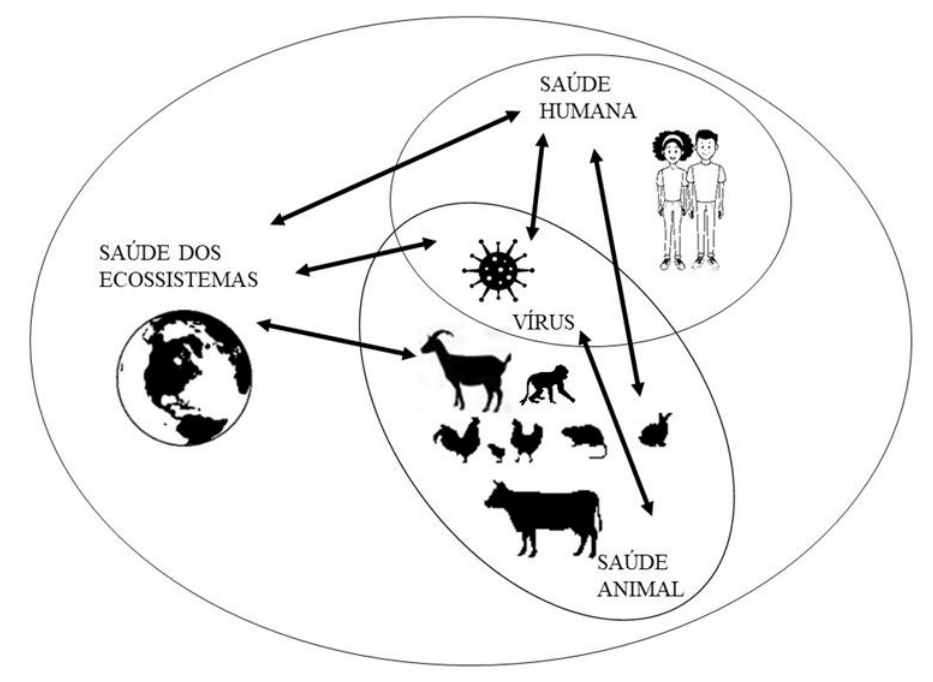
\includegraphics[width=0.95\linewidth]{static/simulados/coluni/figuras/2021/questao-29/figura-1.png}
\end{figure}
% COLUNI-AUTO-FIGURES-END

BONILLA-ALDANA, Katterine et al. Revisiting the One Health approach in the context of COVID-19: a look into the ecology of this emerging disease. \textbf{Advances in Animal Veterinary Science}, v. 8, n. 3, p. 234-237, março, 2020. (Adaptado)

\par

A respeito desse assunto, é INCORRETO afirmar que:



\par



\begin{enumerate}
\item as perturbações da natureza, decorrentes da ocupação inadequada da terra e das alterações
        climáticas, podem levar parasitas, que estão em constante evolução, a infectar novos hospedeiros,
        dando origem às doenças emergentes.
\item o surgimento de novas doenças infecciosas causadas por vírus pode ocorrer a partir de mutações em
        seu material genético, permitindo o contágio de animais silvestres e a transmissão do vírus para o ser
        humano.
\item o consumo de carne de espécies silvestres pode expor o ser humano a novos parasitas e, por isso, é
        um fator importante a ser considerado no surgimento de zoonoses.
\item os vírus são parasitas intracelulares obrigatórios, que infectam células animais sem distinção de
        espécie, parasitando animais silvestres, animais domésticos e também o ser humano.\end{enumerate}
